% Basic slide skeleton for arXiv:2505.20754
\documentclass[aspectratio=169,xcolor=dvipsnames]{beamer}
\usetheme{SimpleDarkBlue}

\usepackage{hyperref}
\usepackage{graphicx}
\usepackage{booktabs}
\usepackage{subcaption}
\usepackage{tikz}
\usepackage[numbers]{natbib}
\usepackage{amsmath,amssymb,amsthm}
\usepackage{pifont}
\usetikzlibrary{arrows.meta,positioning,shapes,calc,decorations.pathreplacing}

\definecolor{graytext}{gray}{0.5}
\definecolor{mmdBlue}{RGB}{25, 96, 170}
\definecolor{mmdGreen}{RGB}{46, 125, 50}
\definecolor{mmdRed}{RGB}{180, 70, 55}
\definecolor{darkgreen}{RGB}{0, 110, 55}
\definecolor{remarkTitle}{RGB}{120, 80, 180}
\definecolor{remarkBody}{RGB}{245, 239, 255}
\newcommand{\red}[1]{\textcolor{red}{#1}}
\newcommand{\blue}[1]{\textcolor{blue}{#1}}
\newcommand{\green}[1]{\textcolor{mmdGreen!80!black}{#1}}
\definecolor{answerBody}{RGB}{255, 236, 210}
\definecolor{assumptionTitle}{RGB}{218, 116, 32}
\definecolor{assumptionBody}{RGB}{255, 241, 222}
\setbeamercolor{answer box}{bg=answerBody, fg=black}
\newenvironment{answer box}{%
    \begin{beamercolorbox}[wd=\linewidth, sep=0.33em, rounded=true]{answer box}%
}{%
    \end{beamercolorbox}%
}
\newcommand{\mmdicon}[2]{%
    \tikz[baseline=(icon.base)]{
        \node[circle, fill=#1, text=white, inner sep=1.2pt, font=\scriptsize\bfseries] (icon) {#2};
    }%
}
\newcommand{\crossedterm}[1]{%
    \tikz[baseline=(term.base)]{
        \node[inner sep=1pt] (term) {\strut #1};
        \draw[mmdRed, line width=1.1pt] (term.west) -- (term.east);
    }%
}
\newcommand{\checkterm}[1]{%
    \tikz[baseline=(term.base)]{
        \node[inner sep=1pt] (term) {\strut #1};
        \draw[mmdGreen!80!black, line width=1.5pt, line cap=round, line join=round]
            ([xshift=-0.25em]term.west) ++(0,0.02em) -- ++(0.18em,-0.18em) -- ++(0.38em,0.42em);
    }%
}
\newcommand{\whycartoon}{%
    
\begin{tikzpicture}[scale=0.92, line cap=round, line join=round]
        \draw[mmdBlue!18, line width=5pt] (-2.25,-0.98) arc[start angle=205,end angle=-25,radius=2.55cm];
        \fill[mmdBlue!9] (0,-0.34) ellipse (1.12cm and 0.50cm);
        \draw[mmdBlue!65!black, line width=1.0pt] (0,-0.34) ellipse (1.12cm and 0.50cm);
        \fill[mmdBlue!8] (0,0.56) circle (0.68cm);
        \draw[mmdBlue!70!black, line width=1.1pt] (0,0.56) circle (0.68cm);
        \draw[mmdBlue!70!black, line width=1.0pt] (-0.28,0.78) -- (-0.05,0.70);
        \draw[mmdBlue!70!black, line width=1.0pt] (0.28,0.78) -- (0.05,0.70);
        \fill[mmdBlue!85!black] (-0.24,0.54) circle (1.5pt);
        \fill[mmdBlue!85!black] (0.24,0.54) circle (1.5pt);
        \draw[mmdBlue!85!black, line width=0.8pt] (-0.18,0.28) .. controls (0,0.20) .. (0.18,0.28);
        \draw[mmdGreen!75!black, line width=1.6pt] (-1.05,-0.22) -- (-0.47,0.08);
        \draw[mmdGreen!75!black, line width=1.2pt] (-1.38,-0.42) circle (0.30cm);
        \draw[mmdRed!80!black, line width=1.1pt, fill=mmdRed!8] (1.10,0.95)
            .. controls (1.10,1.38) and (1.48,1.62) .. (1.90,1.50)
            .. controls (2.35,1.37) and (2.48,0.92) .. (2.20,0.58)
            .. controls (1.96,0.29) and (1.43,0.35) .. (1.22,0.68)
            -- (0.90,0.48) -- (1.06,0.83);
        \node[mmdRed!85!black, font=\Huge\bfseries] at (1.76,0.98) {?};
    \end{tikzpicture}%
}
\newcommand{\sorrycartoon}{%
    
\begin{tikzpicture}[scale=1.15, line cap=round, line join=round]
        \draw[mmdBlue!18, line width=4pt] (-1.25,-1.20) arc[start angle=205,end angle=-25,radius=1.45cm];
        \draw[mmdBlue!65!black, line width=1.1pt] (-0.60,-0.05) -- (0.28,-0.54);
        \draw[mmdBlue!65!black, line width=1.0pt] (-0.28,-0.28) -- (-0.70,-0.62);
        \draw[mmdBlue!65!black, line width=1.0pt] (-0.03,-0.42) -- (0.42,-0.72);
        \draw[mmdBlue!65!black, line width=1.0pt] (0.20,-0.55) -- (0.12,-1.03);
        \draw[mmdBlue!65!black, line width=1.0pt] (0.36,-0.64) -- (0.58,-1.06);
        \fill[mmdBlue!6] (-0.88,0.20) ellipse (0.56cm and 0.42cm);
        \draw[mmdBlue!65!black, line width=1.1pt] (-0.88,0.20) ellipse (0.56cm and 0.42cm);
        \draw[mmdBlue!65!black, line width=1.0pt] (-1.18,0.33) -- (-0.96,0.23);
        \draw[mmdBlue!65!black, line width=1.0pt] (-0.64,0.24) -- (-0.82,0.18);
        \draw[mmdBlue!85!black, line width=0.8pt] (-1.03,0.08) .. controls (-0.89,0.00) .. (-0.73,0.08);
        \draw[mmdGreen!70!black, line width=0.9pt, fill=mmdGreen!15]
            (-0.20,0.48) .. controls (-0.03,0.20) and (-0.12,0.05) .. (-0.30,0.08)
            .. controls (-0.45,0.10) and (-0.47,0.28) .. (-0.20,0.48);
    \end{tikzpicture}%
}
\newcommand{\strengthcartoon}{%
    
\begin{tikzpicture}[scale=1.15, line cap=round, line join=round]
        \fill[mmdBlue!8] (0,0.58) circle (0.62cm);
        \draw[mmdBlue!70!black, line width=1.0pt] (0,0.58) circle (0.62cm);
        \fill[mmdBlue!85!black] (-0.20,0.62) circle (1.5pt);
        \fill[mmdBlue!85!black] (0.20,0.62) circle (1.5pt);
        \draw[mmdBlue!85!black, line width=0.8pt] (-0.16,0.36) .. controls (0,0.18) .. (0.16,0.36);
        \draw[mmdBlue!70!black, line width=1.0pt] (-0.24,0.76) -- (-0.06,0.84);
        \draw[mmdBlue!70!black, line width=1.0pt] (0.24,0.76) -- (0.06,0.84);
    \end{tikzpicture}%
}
\newcommand{\limitationcartoon}{%
    
\begin{tikzpicture}[scale=1.15, line cap=round, line join=round]
        \fill[mmdBlue!8] (0,0.58) circle (0.62cm);
        \draw[mmdBlue!70!black, line width=1.0pt] (0,0.58) circle (0.62cm);
        \fill[mmdBlue!85!black] (-0.20,0.62) circle (1.5pt);
        \fill[mmdBlue!85!black] (0.20,0.62) circle (1.5pt);
        \draw[mmdBlue!85!black, line width=0.8pt] (-0.18,0.44) .. controls (0,0.25) .. (0.18,0.44);
        \draw[mmdBlue!70!black, line width=1.0pt] (-0.24,0.82) -- (-0.08,0.74);
        \draw[mmdBlue!70!black, line width=1.0pt] (0.24,0.82) -- (0.08,0.74);
    \end{tikzpicture}%
}


% Render slide citations as compact grey alphabetic labels.
\let\oldcitep\citep
\let\oldcitet\citet
\renewcommand{\citep}[1]{{\scriptsize\textcolor{graytext}{\oldcitep{#1}}}}
\renewcommand{\citet}[1]{{\scriptsize\textcolor{graytext}{\oldcitet{#1}}}}
\renewcommand{\cite}[1]{{\scriptsize\textcolor{graytext}{\oldcitep{#1}}}}

\title{Stationary MMD Points}
\subtitle{ICML 2026}
\author{Zonghao (Hudson) Chen}
\institute{}
\date{}

\newtheorem{thm}{Theorem}
\newtheorem*{thm*}{Theorem}
\newtheorem{lem}[thm]{Lemma}
\newtheorem{prop}[thm]{Proposition}
\newtheorem{defi}{Definition}
\newtheorem{assumptionthm}{Assumption}
\newenvironment{assumption}[1][]{%
    \begingroup
    \setbeamercolor{block title}{bg=assumptionTitle, fg=white}%
    \setbeamercolor{block body}{bg=assumptionBody, fg=black}%
    \if\relax\detokenize{#1}\relax
        \begin{assumptionthm}%
    \else
        \begin{assumptionthm}[#1]%
    \fi
}{%
    \end{assumptionthm}%
    \endgroup
}
\newenvironment{rem}{%
    \begingroup
    \setbeamercolor{remark box}{bg=remarkBody, fg=black}%
    \begin{beamercolorbox}[wd=\linewidth, sep=0.33em, rounded=true]{remark box}%
    \textbf{\textcolor{remarkTitle}{Remark.}}\hspace{0.4em}
}{%
    \end{beamercolorbox}%
    \endgroup
}

\begin{document}

\newcommand{\E}{\mathbb{E}}
\newcommand{\R}{\mathbb{R}}
\newcommand{\Qb}{\mathbb{Q}}
\newcommand{\Pb}{\mathbb{P}}
\newcommand{\calH}{\mathcal{H}}
\newcommand{\calE}{\mathcal{E}}
\newcommand{\calT}{\mathcal{T}}
\newcommand{\calL}{\mathcal{L}}
\newcommand{\calI}{\mathcal{I}}
\newcommand{\calF}{\mathcal{F}}
\newcommand{\calG}{\mathcal{G}}
\newcommand{\calZ}{\mathcal{Z}}
\newcommand{\calO}{\mathcal{O}}
\newcommand{\calY}{\mathcal{Y}}
\newcommand{\calX}{\mathcal{X}}
\newcommand{\calP}{\mathcal{P}}
\newcommand{\calN}{\mathcal{N}}
\newcommand{\calB}{\mathcal{B}}
\newcommand{\dd}{\mathrm{d}}
\newcommand{\bx}{\mathbf{x}}
\newcommand{\bo}{\mathbf{o}}
\newcommand{\by}{\mathbf{y}}
\newcommand{\bz}{\mathbf{z}}
\newcommand{\bH}{\mathbf{H}}
\newcommand{\bw}{\mathbf{w}}
\newcommand{\bJ}{\mathbf{J}}
\newcommand{\bomega}{\boldsymbol{\omega}}
\newcommand{\bnabla}{\boldsymbol{\nabla}}
\newcommand{\scrG}{\mathscr{G}}
\newcommand{\scrF}{\mathscr{F}}
\newcommand{\scrX}{\mathscr{X}}
\newcommand{\scrx}{\mathscr{X}}
\newcommand{\scrY}{\mathscr{Y}}
\newcommand{\scry}{\mathscr{Y}}
\newcommand{\scrH}{\mathscr{H}}
\newcommand{\scrZ}{\mathscr{Z}}
\newcommand{\scrz}{\mathscr{Z}}
\newcommand{\scrU}{\mathscr{U}}
\newcommand{\scrR}{\mathscr{R}}
\newcommand{\scrQ}{\mathscr{Q}}
\newcommand{\mmd}{\operatorname{MMD}}
\newcommand{\op}{\operatorname{op}}

\newcommand{\Id}{\mathrm{Id}}
\newcommand{\N}{\mathbb{N}}
\newcommand{\kl}{\mathrm{KL}}
\newcommand{\LSI}{\mathrm{LSI}}

\newcommand{\bm}[1]{\boldsymbol{#1}}

\newcommand{\Var}{\operatorname{Var}}

\newcommand{\textfrac}[2]{{\textstyle\frac{#1}{#2}}}

\newcommand{\kts}{\textsc{kt-split}\xspace}
\newcommand{\ktsc}{\textsc{kt-split}-Compress\xspace}
\newcommand{\ktscd}[1][\delta]{\textsc{kt-split}-Compress$(#1)$\xspace}
\newcommand{\ktc}{KT-Compress\xspace}
\newcommand{\ktcd}{KT-Compress$(\delta)$\xspace}

\newcommand{\event}{\mathcal{E}}
\newcommand{\eventd}{\event(\delta)}
\def\norm#1{\|{#1}\|} % A norm with 1 argument

\def\indic#1{\mathbbm{1}_{#1}} % Indicator function

\begin{frame}
  \titlepage
\end{frame}

\section{Personal}
\begin{frame}{About Me}
    \vspace{-0.25cm}
    \begin{columns}[T,onlytextwidth]
        \column{0.34\textwidth}
        \begin{minipage}[t][0.68\textheight][t]{\linewidth}
            \centering
            
\begin{tikzpicture}
                \node[
                    draw=mmdBlue!55!black,
                    line width=0.8pt,
                    rounded corners=4pt,
                    inner sep=2.5pt
                ] {
                    \IfFileExists{figures/personal.pdf}{
                      \includegraphics[width=0.86\linewidth,height=0.58\textheight,keepaspectratio]{figures/personal.pdf}
                    }{
                      \begin{minipage}[c][0.58\textheight][c]{0.86\linewidth}
                        \centering\small\color{graytext}Add personal photo at\\figures/personal.pdf
                      \end{minipage}
                    }
                };
            \end{tikzpicture}
        \end{minipage}

        \column{0.62\textwidth}
        {\Large\bfseries Zonghao (Hudson) Chen}\\[-0.04cm]
        {\small\color{graytext}4th year PhD student, University College London}\\[0.22cm]

        \begin{beamercolorbox}[wd=\linewidth, sep=0.33em, rounded=true]{answer box}
            \small
            \begin{tabular}{@{}p{0.44\linewidth}p{0.46\linewidth}@{}}
                Foundational AI Centre & Fran\c{c}ois-Xavier Briol\\
                Gatsby Unit & Arthur Gretton
            \end{tabular}
        \end{beamercolorbox}

        \vspace{0.18cm}
        \begin{beamercolorbox}[wd=\linewidth, sep=0.33em, rounded=true]{answer box}
            \small
            Tsinghua Uni., B.Eng. in Electronic Engineering, 2022
        \end{beamercolorbox}

        \vspace{0.18cm}
        \begin{beamercolorbox}[wd=\linewidth, sep=0.33em, rounded=true]{answer box}
            {\bfseries Research Interests}\\
            \small
            \vspace{-0.14cm}
            \begin{itemize}
                \setlength\topsep{0pt}
                \setlength\partopsep{0pt}
                \setlength\parsep{0pt}
                \setlength\itemsep{0.02cm}
                \item Kernel and nonparametric methods
                \item Statistical learning theory
            \end{itemize}
            \vspace{-0.26cm}
        \end{beamercolorbox}
    \end{columns}
\end{frame}

\begin{frame}{Motivation}
    \begin{exampleblock}{}
        \textbf{Problem:} Approximation of a target distribution $\mu$ with a finite set of points $\{x_i\}_{i=1}^n$.
    \end{exampleblock}
    \begin{columns}[T,onlytextwidth]
        \column{0.59\textwidth}

        \begin{itemize}
            \item Denote the empirical distribution of $\{x_i\}_{i=1}^n$ as 
            $$\mu_n = \frac{1}{n}\sum_{i=1}^n \delta_{x_i}.$$
            \item We want $\mu_n$ to be close to $\mu$.
        \end{itemize}

        \column{0.39\textwidth}
        \centering
        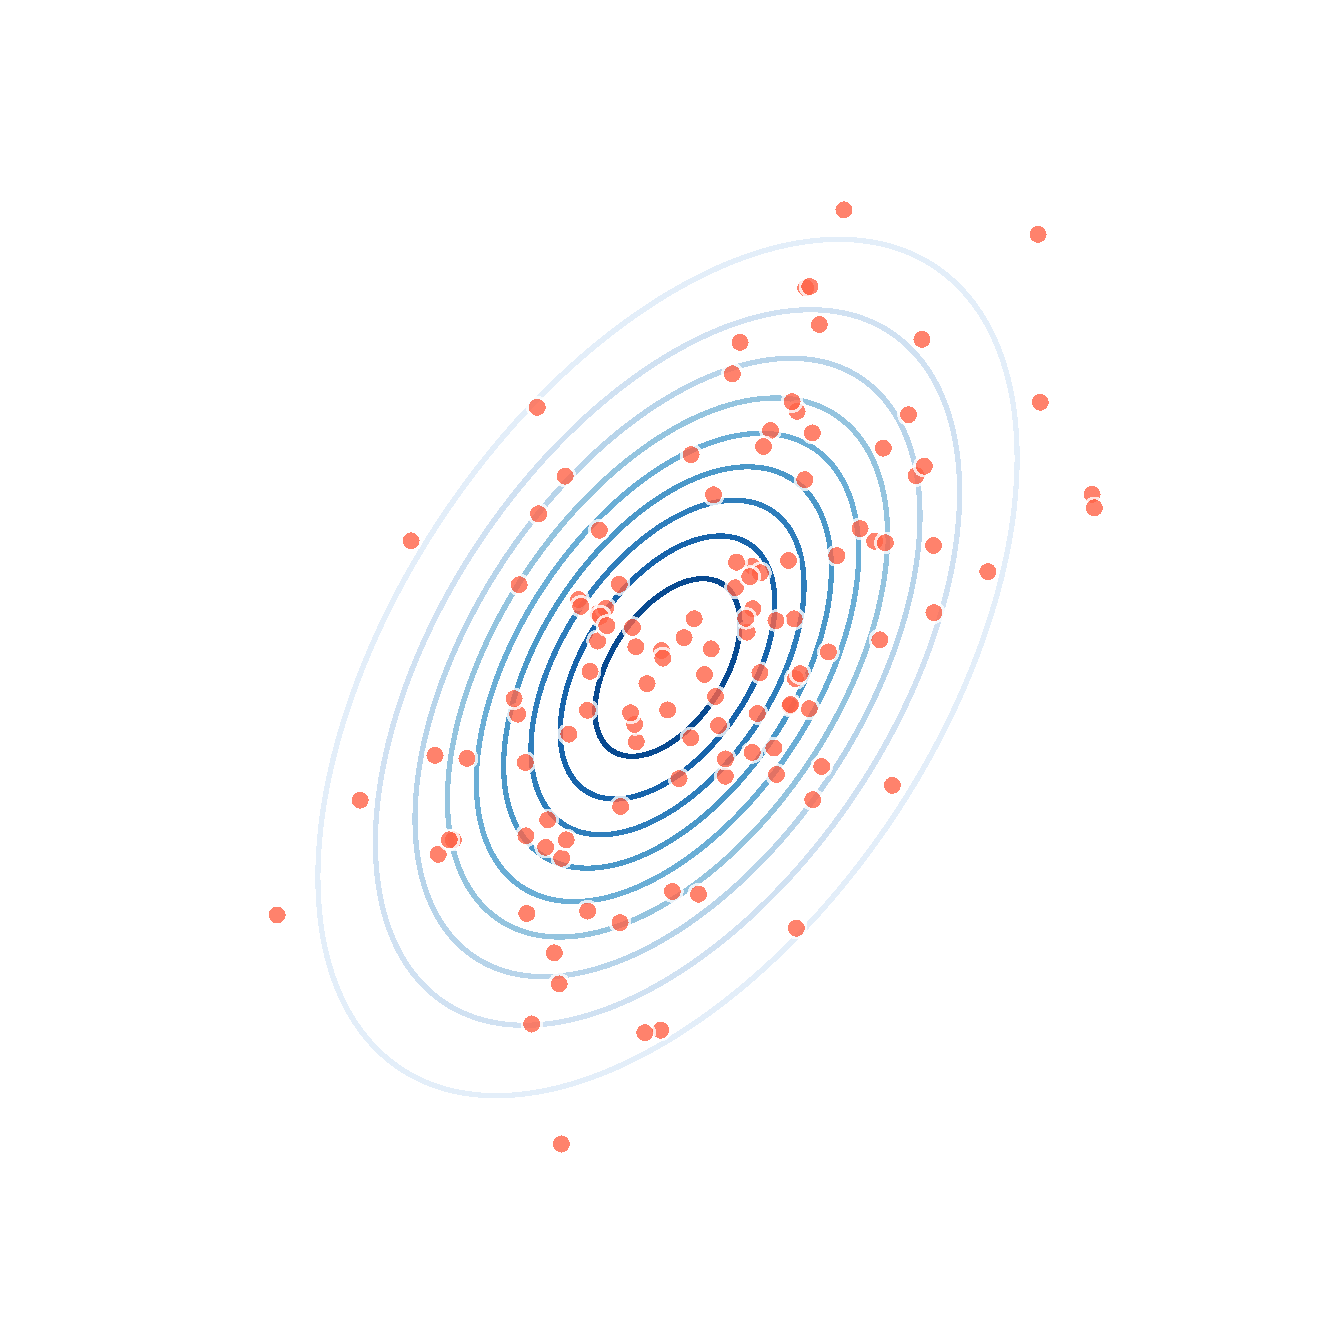
\includegraphics[width=\linewidth,trim=18 18 18 18,clip]{figures/gaussian_mu_samples.pdf}
    \end{columns}
\end{frame}

\begin{frame}{Motivation}
    \centering
    \begin{exampleblock}{}
        \textbf{Problem:} Approximation of a target distribution $\mu$ with a finite set of points $\{x_i\}_{i=1}^n$.
    \end{exampleblock}
    \vspace{0.25cm}
    \begin{columns}[T,onlytextwidth]
        \column{0.31\textwidth}
        \centering
        \setlength{\fboxsep}{5pt}
        \vspace{0pt}%
        \fcolorbox{mmdGreen!65!black}{mmdGreen!8}{%
            \begin{minipage}[t][0.40\textheight][t]{0.88\linewidth}
                \centering
                {\Large \mmdicon{mmdGreen!80!black}{$\int$}}\\[0.08cm]
                {\bfseries Numerical Integration}\\[0.10cm]
                \vspace{0.2cm}
                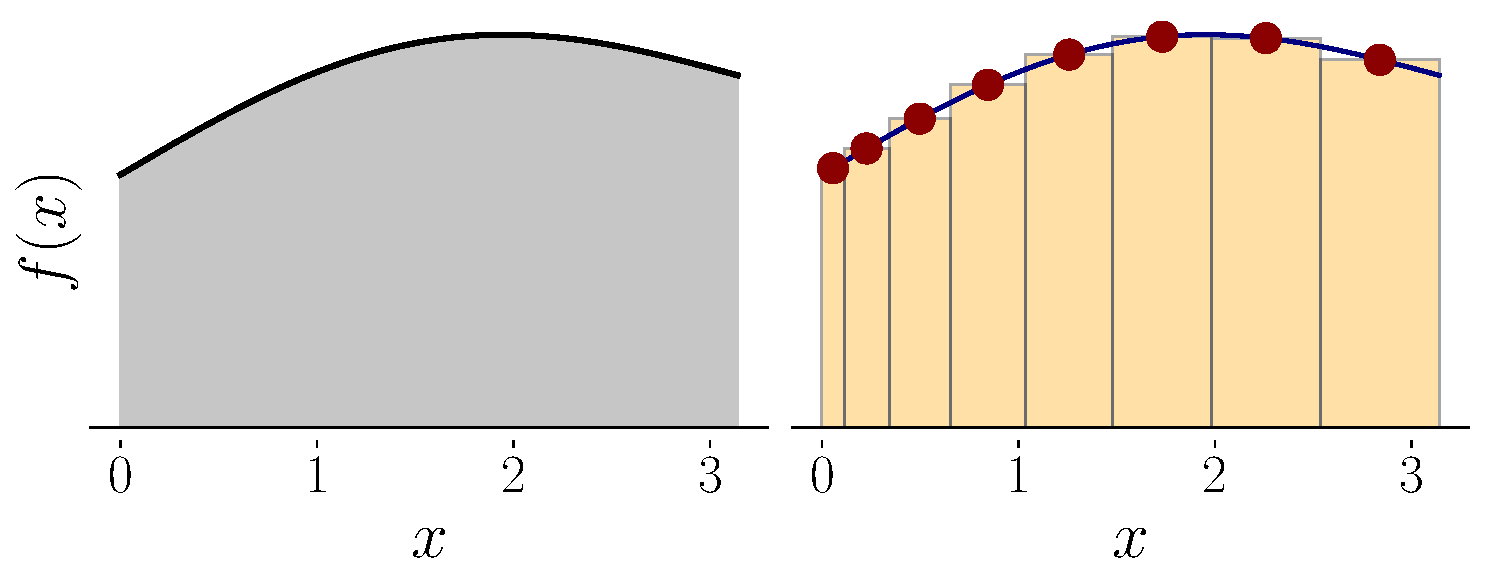
\includegraphics[width=\linewidth,height=0.20\textheight,keepaspectratio]{figures/integral_illustration.pdf}
            \end{minipage}
        }

        \column{0.31\textwidth}
        \centering
        \setlength{\fboxsep}{5pt}
        \vspace{0pt}%
        \fcolorbox{mmdBlue!70!black}{mmdBlue!8}{%
            \begin{minipage}[t][0.40\textheight][t]{0.88\linewidth}
                \centering
                {\Large \mmdicon{mmdBlue!80!black}{$\sim$}}\\[0.08cm]
                {\bfseries Sampling}\\[0.10cm]
                \vspace{0.2cm}
                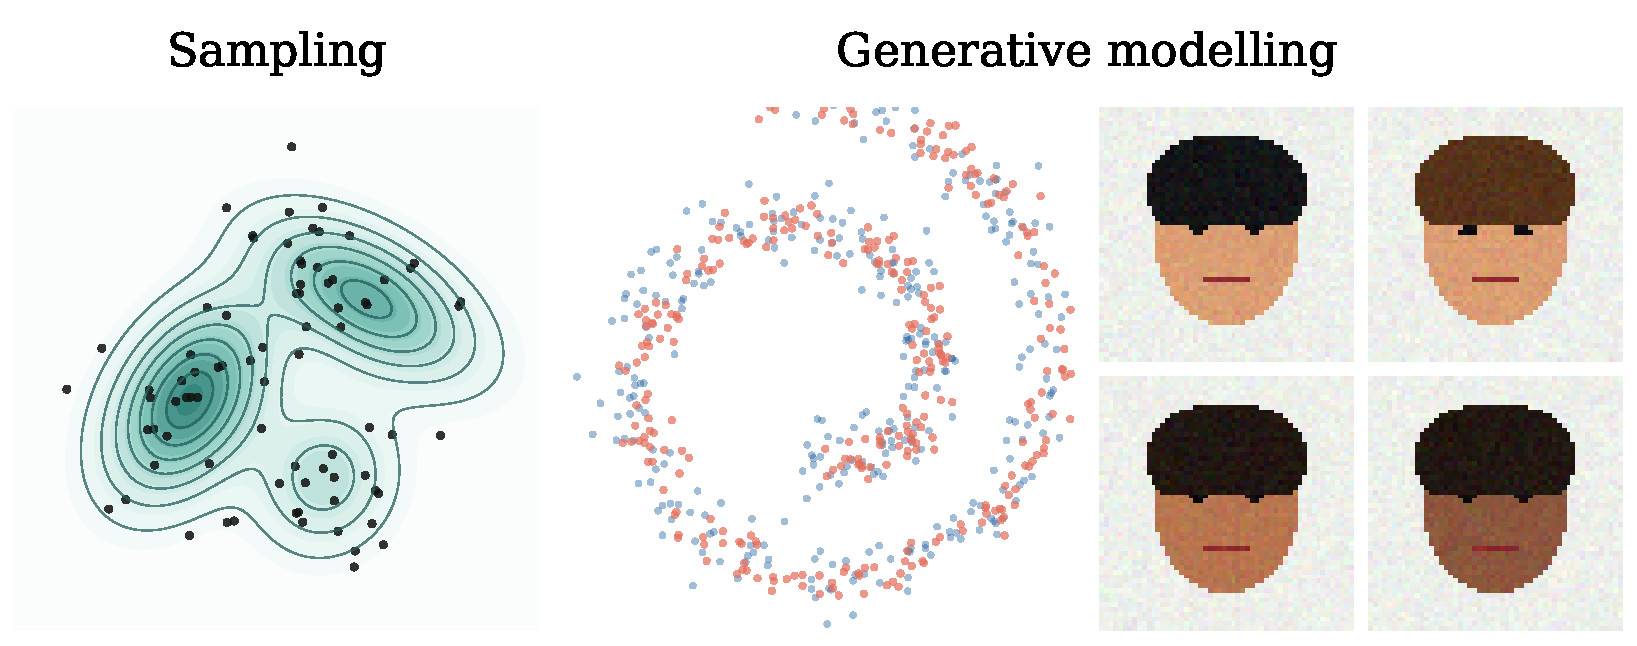
\includegraphics[width=\linewidth,height=0.20\textheight,keepaspectratio]{figures/sampling_generative_illustration.pdf}
            \end{minipage}
        }

        \column{0.31\textwidth}
        \centering
        \setlength{\fboxsep}{5pt}
        \vspace{0pt}%
        \fcolorbox{mmdRed!70!black}{mmdRed!8}{%
            \begin{minipage}[t][0.40\textheight][t]{0.88\linewidth}
                \centering
                {\Large \mmdicon{mmdRed!80!black}{$\mathcal{C}$}}\\[0.08cm]
                {\bfseries Coreset Selection}\\[0.10cm]
                \vspace{0.2cm}
                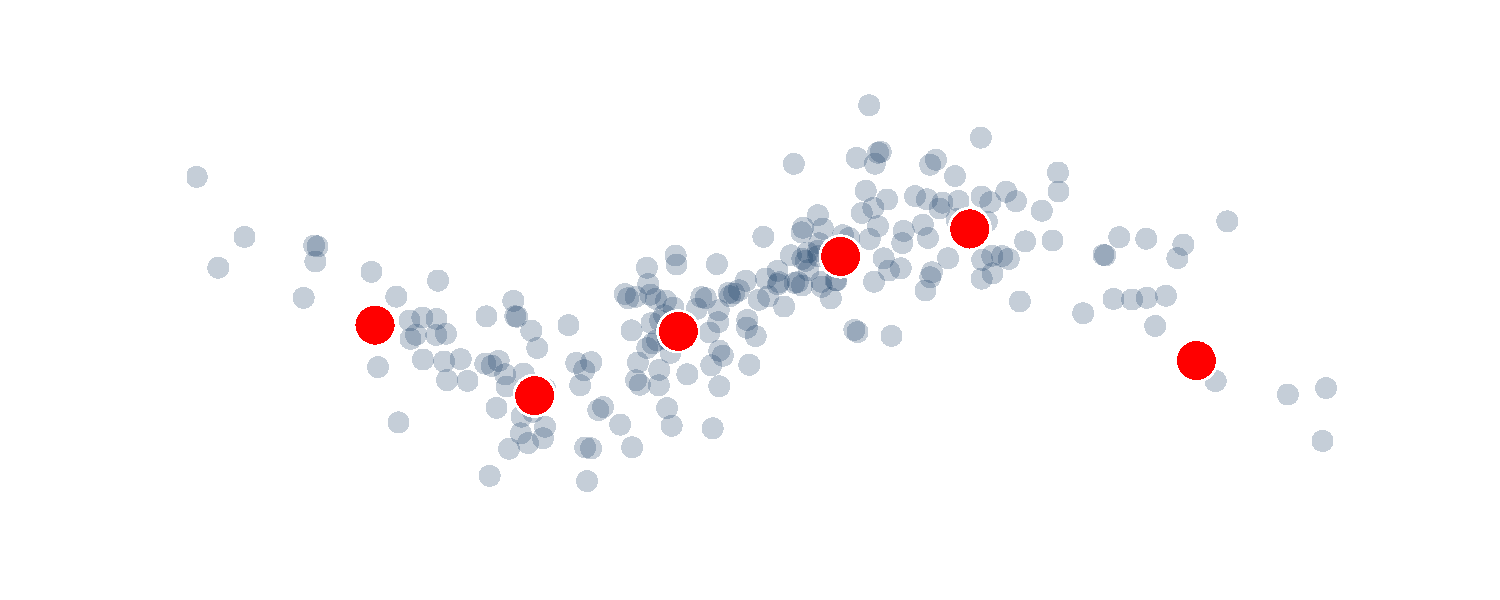
\includegraphics[width=\linewidth,height=0.20\textheight,keepaspectratio]{figures/coreset_selection_illustration.pdf}
            \end{minipage}
        }
    \end{columns}
\end{frame}

\begin{frame}{An empirical observation}
    \begin{center}
        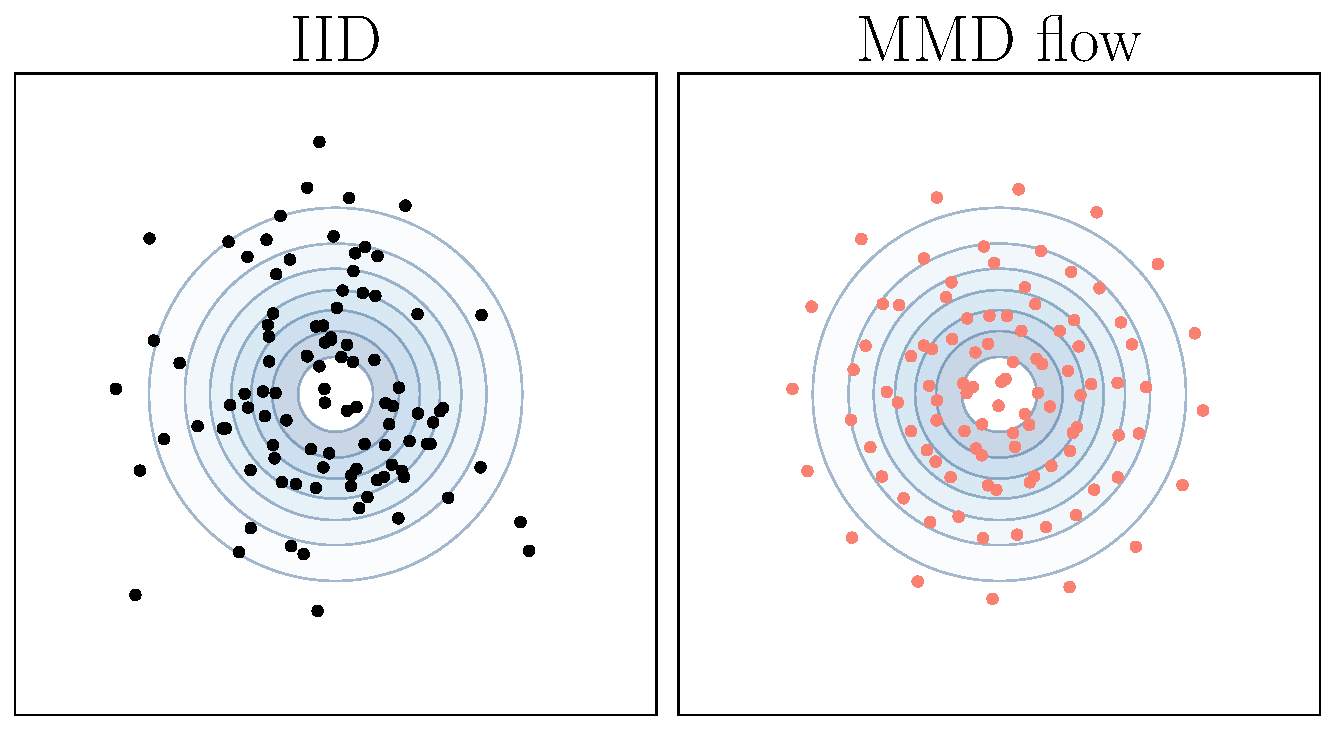
\includegraphics[height=0.40\textheight,keepaspectratio]{figures/sampling_gaussian_two_panel_summary.pdf}%
        \hspace{0.18cm}%
        \raisebox{-0.079\textheight}{%
            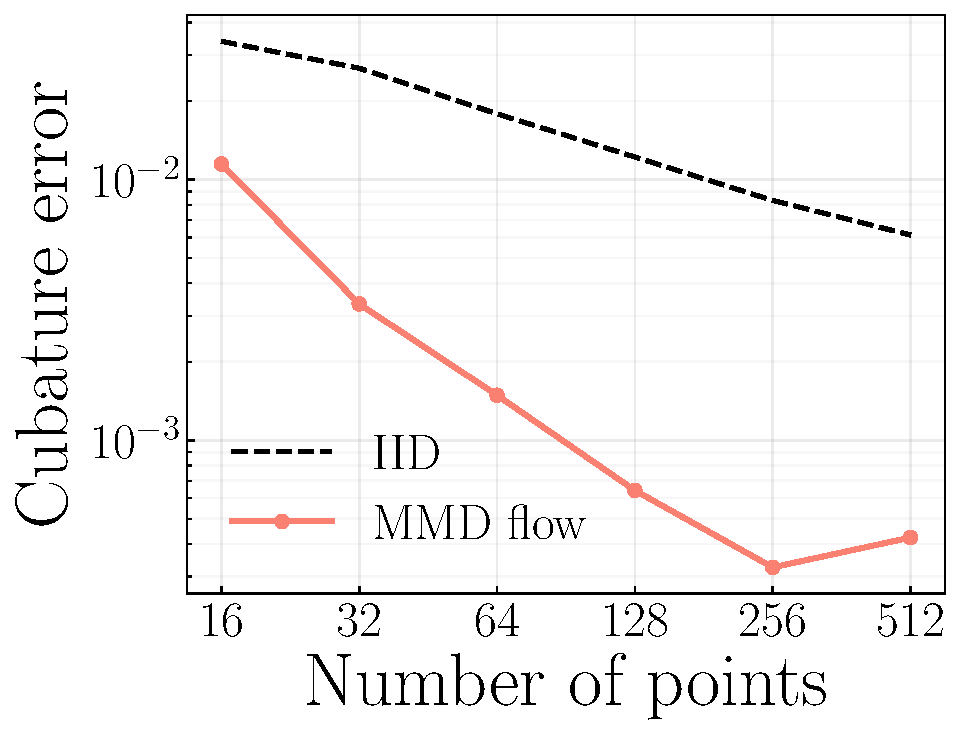
\includegraphics[height=0.445\textheight,keepaspectratio]{figures/gaussian_cubature_error.pdf}%
        }%
    \end{center}
    \begin{itemize}
        \item Samples from MMD flow are more \textcolor{mmdGreen!80!black}{uniform} than IID samples~\citep{xu2022accurate}.
        \item Lower numerical integration error for fixed $n$.
        \begin{align*}
            \left| \int f(x) \; \dd \mu(x) - \int f(x) \; \dd \mu_n(x) \right| . 
        \end{align*}
    \end{itemize}
    \vspace{-0.1cm}
    \begin{exampleblock}{}
        \centering \textbf{Goal:} Why? 
    \end{exampleblock}
\end{frame}

\begin{frame}{Background: What is MMD?}
    \begin{columns}[c]
        \column{0.50\textwidth}
        \begin{itemize}
            \item Given two distributions $\Pb$ and $\Qb$, how to compare them? 
            \item $|\E_{\Pb}[X] - \E_{\Qb}[X]|$. 
            \item $|\E_{\Pb}[X^2] - \E_{\Qb}[X^2]|$.
            \item The first two moments are not enough! 
        \end{itemize}

        \column{0.5\textwidth}
        \centering
        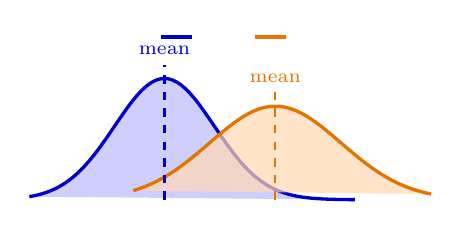
\begin{tikzpicture}[scale=0.88, every node/.style={font=\scriptsize}]
            \draw[blue!80!black, very thick] (-0.8,2.35) -- (-0.35,2.35)
                node[right, black] {$\Pb$};
            \draw[orange!90!black, very thick] (0.55,2.35) -- (1.0,2.35)
                node[right, black] {$\Qb$};

            \fill[blue!25, opacity=0.75]
                plot[smooth, samples=100, domain=-2.7:2.0]
                (\x,{1.75*exp(-0.5*((\x+0.75)/0.72)^2)});
            \draw[blue!80!black, very thick]
                plot[smooth, samples=100, domain=-2.7:2.0]
                (\x,{1.75*exp(-0.5*((\x+0.75)/0.72)^2)});

            \fill[orange!30, opacity=0.7]
                plot[smooth, samples=100, domain=-1.2:3.1]
                (\x,{1.35*exp(-0.5*((\x-0.85)/0.95)^2)});
            \draw[orange!90!black, very thick]
                plot[smooth, samples=100, domain=-1.2:3.1]
                (\x,{1.35*exp(-0.5*((\x-0.85)/0.95)^2)});

            \draw[blue!80!black, dashed, thick] (-0.75,0) -- (-0.75,1.95)
                node[above] {mean};
            \draw[orange!90!black, dashed, thick] (0.85,0) -- (0.85,1.55)
                node[above] {mean};

        \end{tikzpicture}
    \end{columns}
    \vspace{0.3cm}
    \begin{exampleblock}{}
\centering
    \textbf{Goal}: Compare $\Pb$ and $\Qb$ with a general $f$, i.e., $|\E_{\Pb}[f(X)] - \E_{\Qb}[f(X)]|$?
\end{exampleblock}
\end{frame}

\begin{frame}{Background: Maximum Mean Discrepancy (MMD)~\citep{gretton2012kernel}}
    \begin{columns}[c]
        \column{0.8\textwidth}
        \begin{itemize}
            \item $\calH$ is a reproducing kernel Hilbert space (RKHS) with kernel $k$.
            \begin{align*}
                \text{MMD}(\Pb, \Qb)
                := \sup_{f \in \calH}
                |\E_{\Pb}[f(X)] - \E_{\Qb}[f(X)]|.
            \end{align*}
            \item The RKHS contains functions that are linear combinations of the feature maps $\phi:\calX\to\calH$, $f=\sum_{i=1}^n \alpha_i \phi(x_i)$.

        \end{itemize}

        \column{0.2\textwidth}
        \centering
        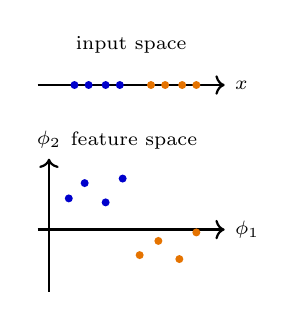
\begin{tikzpicture}[scale=0.72, every node/.style={font=\scriptsize}]
            \begin{scope}
                \draw[->, thick] (-1.55,0) -- (1.75,0) node[right] {$x$};
                \node[above] at (0.1,0.38) {input space};

                \foreach \x in {-0.9,-0.65,-0.35,-0.1} {
                    \fill[blue!80!black] (\x,0) circle (2pt);
                }
                \foreach \x in {0.45,0.7,1.0,1.25} {
                    \fill[orange!90!black] (\x,0) circle (2pt);
                }
                \node[blue!80!black] at (-0.55,-0.35) {$\Pb$};
                \node[orange!90!black] at (0.95,-0.35) {$\Qb$};
            \end{scope}
            \vspace{0.2cm}
            \begin{scope}[shift={(0,-2.55)}]
                \draw[->, thick] (-1.55,0) -- (1.75,0) node[right] {$\phi_1$};
                \draw[->, thick] (-1.35,-1.1) -- (-1.35,1.25) node[above] {$\phi_2$};
                \node[above] at (0.15,1.25) {feature space};

                \foreach \p in {(-1.0,0.55),(-0.72,0.82),(-0.35,0.48),(-0.05,0.9)} {
                    \fill[blue!80!black] \p circle (2pt);
                }
                \foreach \p in {(0.25,-0.45),(0.58,-0.2),(0.95,-0.52),(1.25,-0.05)} {
                    \fill[orange!90!black] \p circle (2pt);
                }
            \end{scope}
        \end{tikzpicture}
    \end{columns}
    \begin{thm*}
        MMD admits a closed-form expression:
        \begin{align*}
            \mathrm{MMD}^2(\Pb, \Qb)
            = \E_{X,X'\sim\Pb}[k(X,X')]
            + \E_{Y,Y'\sim\Qb}[k(Y,Y')] - 2\E_{X\sim\Pb,\,Y\sim\Qb}[k(X,Y)] .
        \end{align*}
    \end{thm*}
    \begin{itemize}
        \item MMD is a probability divergence ($\mathrm{MMD}(\Pb, \Qb)=0 \iff \Pb=\Qb$) if $k$ is $c_0$-universal (Gaussian)~\citep{sriperumbudur2011universality}.
    \end{itemize}
\end{frame}


\begin{frame}{Background: MMD gradient flow~\citep{arbel2019maximum}}
    \vspace{-0.15cm}
    \begin{itemize}
        \setlength\itemsep{0.05cm}
        \item Start with an initial set of $n$ particles $\{x_i^{(0)}\}_{i=1}^n$ at time $0$.
        \item Evolve the particles according to the MMD gradient flow:
        \begin{align*}
            x_i^{(t+1)} = x_i^{(t)} - \gamma \cdot \nabla_{x_i^{(t)}} 
            \mathrm{MMD}^2\left(\mu, \frac{1}{n} \sum_{j=1}^n \delta_{x_j^{(t)}}\right), \qquad i=1,\ldots,n.
        \end{align*}
        \vspace{-0.6cm}
        \begin{itemize}
            \item $\gamma>0$ is the step size.
        \end{itemize}
    \end{itemize}
    \vspace{0.3cm}
    \centering
    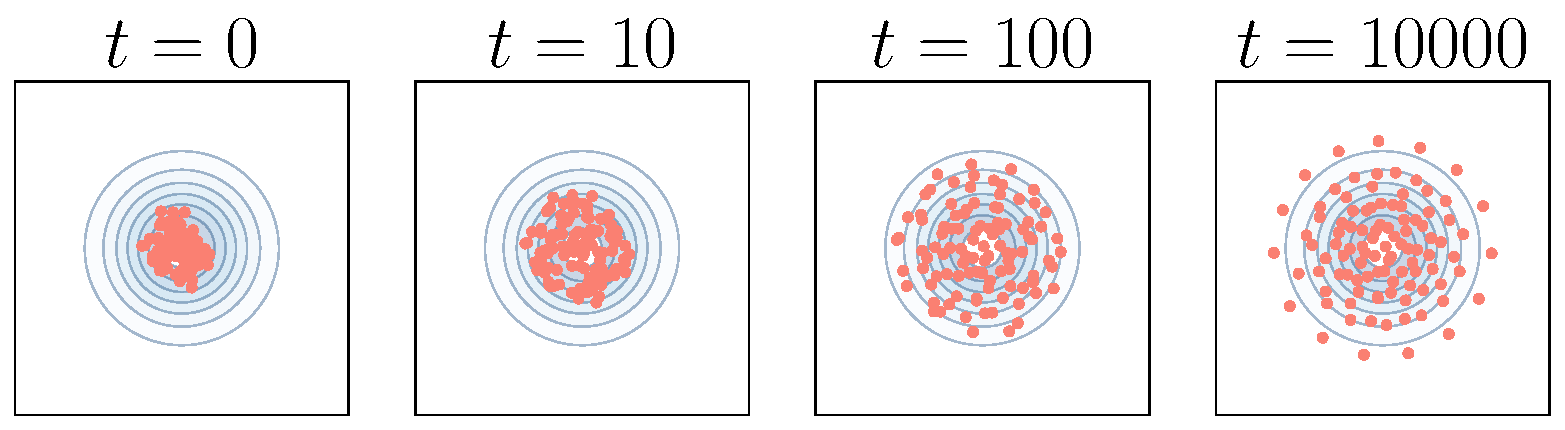
\includegraphics[width=0.9\linewidth,height=0.34\textheight,keepaspectratio]{figures/sampling_gaussian_mmd_flow_trajectory.pdf}
    \begin{itemize}
        \item A Wasserstein gradient flow.
    \end{itemize}
\end{frame}


\begin{frame}{Motivation}
    \begin{exampleblock}{}
        \centering \textbf{Observation:} MMD flow samples are more \textcolor{mmdGreen!80!black}{uniform} than IID samples~\citep{xu2022accurate}.
    \end{exampleblock}
    \vspace{0.35cm}
    \centering
    \whycartoon
\end{frame}

\begin{frame}{Existing work}
    \begin{itemize}
        \item Existing finite-sample rates in MMD gradient flows~\citep{arbel2019maximum,chen2025drmmd}.
        \item Let ${\mu}_n^{(t)}=\frac{1}{n} \sum_{j=1}^n \delta_{x_j^{(t)}}$ be the empirical distribution of $n$ particles at iterate $t$. 
        \begin{align*}
            \mmd\left(\mu, {\mu}_n^{(t)}\right) \leq C(t) n^{-\frac{1}{2}}, 
            \quad W_2\left(\mu, {\mu}_n^{(t)}\right) 
            \leq C(t) n^{-\frac{1}{2}}.
        \end{align*}
    \end{itemize}
    \begin{answer box}
        {\centering\textbf{Limitations}\par}
        \begin{itemize}
            \item Same rate as IID sampling: $n^{-\frac{1}{2}}$.
            \item The constant $C(t)$ grows exponentially in $t$. 
        \end{itemize}
    \end{answer box}
\end{frame}

\begin{frame}{Existing work}
    \begin{itemize}
        \item Minimum MMD points
        \vspace{-0.4cm}
        \begin{align*}
            \{x_i^*\}_{i=1}^n = \arg\min_{\{x_i\}_{i=1}^n} \operatorname{MMD}^2\left(\mu, \frac{1}{n} \sum_{j=1}^n \delta_{x_j}\right).
        \end{align*}
        \vspace{-0.4cm}
        \item Let ${\mu}_n^{\ast}=\frac{1}{n} \sum_{j=1}^n \delta_{x_j^{\ast}}$ 
        be the empirical distribution~\citep{xu2022accurate,dick2010digital}: 
        \vspace{-0.2cm}
        \begin{align*}
            \mmd\left(\mu, {\mu}_n^{\ast} \right) \leq C n^{-1}.
        \end{align*}
        \vspace{-0.6cm}
        \item Quasi Monte Carlo point set achieve this rate~\citep{dick2010digital}.
    \end{itemize}
    \vspace{0.1cm}
    \begin{answer box}
        {\centering\textbf{Limitations}\par}
        \begin{itemize}
            \item Minimum MMD points are hard to compute, due to the non-convexity of MMD.
            \item Gradient descent only finds a \textcolor{mmdRed}{stationary} point instead.
        \end{itemize}
    \end{answer box}
\end{frame}

\begin{frame}{Motivation}
    \centering
    {\large
        \textcolor{mmdRed}{$\times$}\,
        \crossedterm{\textbf{Minimum MMD points}}
        \quad{\color{graytext}but}\quad
        \textcolor{mmdGreen!80!black}{$\checkmark$}\,
        \textbf{Stationary MMD points}
    }\\[0.16cm]

    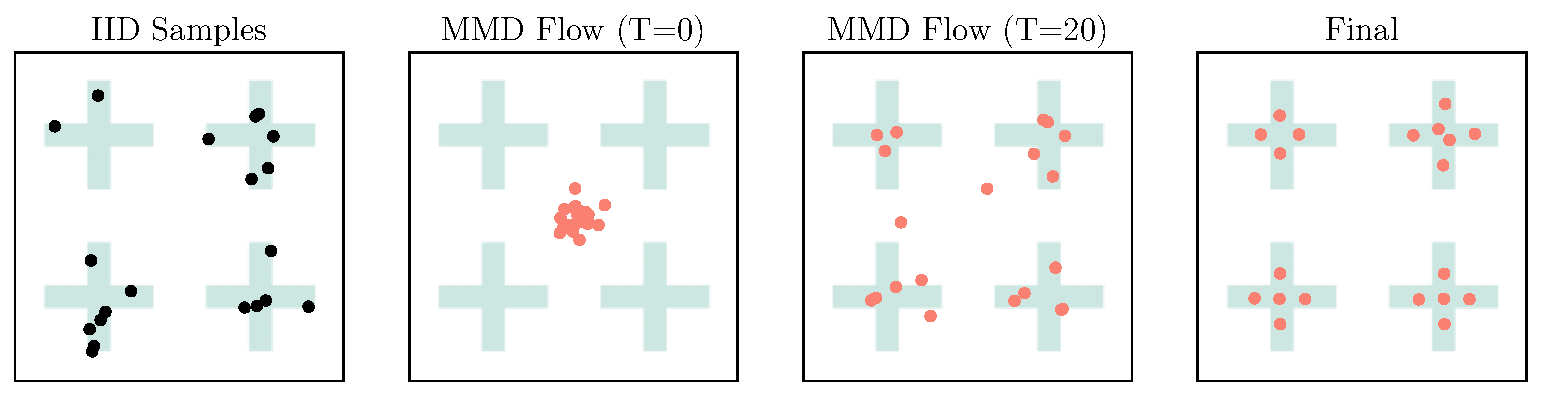
\includegraphics[width=0.94\linewidth]{figures/illustration_stationary.pdf}
    \begin{itemize}
        \item A four-cross distribution.
        \item An ideal minimum MMD points would have $5$ points in each cross.
        \item Stationary MMD points have $(4,6,5,5)$ points in each cross.
    \end{itemize}
\end{frame}

\begin{frame}{Stationary MMD points}
    \begin{defi}[Stationary MMD points]
        A sequence of point sets $\{x_i\}_{i=1}^n$ with
        $\mu_n := \frac{1}{n}\sum_{i=1}^n \delta_{x_i}$, that satisfies:
        \begin{enumerate}
            \item \textbf{\red{Convergence:}}
            $\mmd(\mu,\mu_n)\to 0$ as $n\to\infty$.
            \item \textbf{\blue{Stationarity:}}
            $\nabla_{x_1,\ldots,x_n}\mmd^2(\mu,\mu_n)=0$.
        \end{enumerate}
    \end{defi}
    \begin{itemize}
        \item Minimum MMD points are a special case of stationary MMD points.
        \item Stationary MMD points are easier to compute, e.g., via MMD gradient flow.
    \end{itemize}
    \vspace{0.3cm}
    \begin{exampleblock}{}
        \centering \textbf{Question:} Why does stationary MMD points exhibit superior numerical integraion performance than IID points?
    \end{exampleblock}
\end{frame}

\begin{frame}{Stationary MMD points}
\begin{itemize}
    \item Simulate MMD flow for long enough, $t\to\infty$. 
    \item For any $i\in\{1, \ldots, n\}$:  
\begin{align*}
    \nabla_{x_i} \operatorname{MMD}^2\left(\mu, \; \frac{1}{n} \sum_{j=1}^n \delta_{x_j}\right)=0 
    \Longrightarrow \frac{1}{n} \sum_{j=1}^n \nabla_1 k\left(x_i, x_j\right)-\int \nabla_1 k\left(x_i, y\right) \mathrm{d} \mu(y)=0. 
\end{align*}
    \item Exact integration on $x \mapsto \nabla_1 k\left(x_i, x\right)$.
    \item Exact integration on $\{1\}$.
\end{itemize}
\begin{exampleblock}{}
    \centering \textbf{Exact integration subspace:} 
    \vspace{-0.20cm}
    \begin{align*}
    \mathcal{F}_n := \operatorname{span}\Bigl(
    \{1\} \cup \bigl\{\nabla_1 k(x_i,\cdot) : i\in\{1, \ldots, n\}\bigr\}
    \Bigr) \subset \mathcal{H}.
    \end{align*}
\end{exampleblock}
\end{frame}

\begin{frame}{Stationary MMD points}
    \centering
    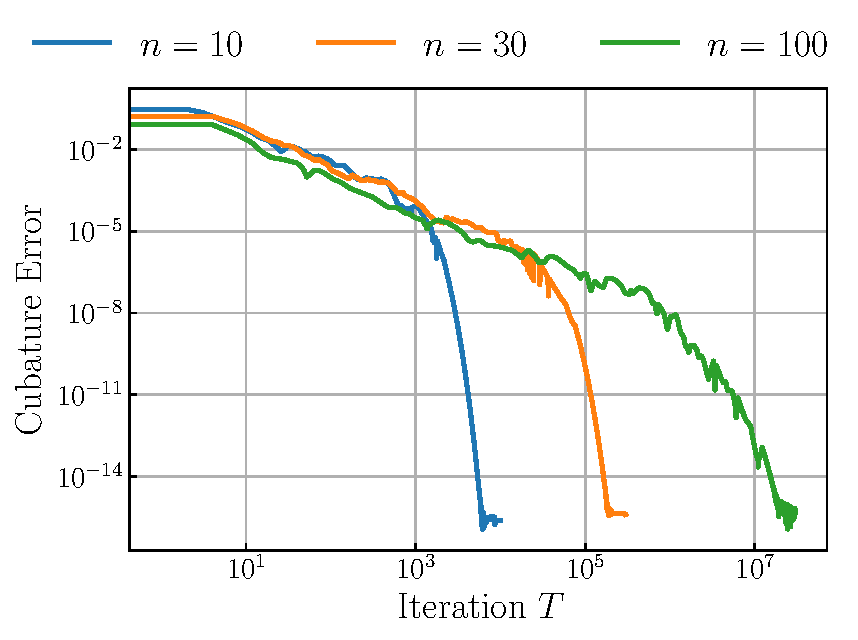
\includegraphics[width=0.5\linewidth,height=0.80\textheight,keepaspectratio]{figures/exactness.pdf}
    \begin{itemize}
        \item Exact integration on $\calF_n$.
    \end{itemize}
\end{frame}

\begin{frame}{Stationary MMD points}
\begin{assumption}
    The kernel $k$ is smooth and $c_0$-universal.
\end{assumption}

\begin{prop}[Approximation of $\calF_n$ towards $\calH$]
Given $f\in\calH$. Consider the semi-norm
$$
|f|_n:=\inf \left\{\left\|r_n\right\|_{\mathcal{H}}: f=f_n+r_n, \; f_n \in \mathcal{F}_n, \; r_n \in \mathcal{H}\right\}
$$
Then, $\lim _{n \rightarrow \infty}|f|_n=0$.
\end{prop}

\vspace{0.3cm}
\centering
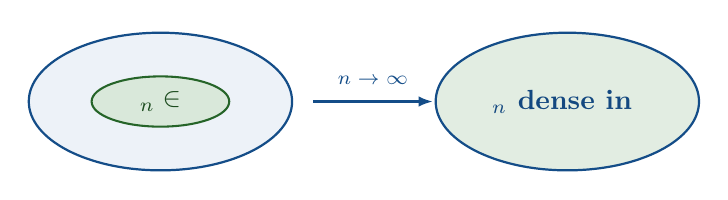
\begin{tikzpicture}[
    scale=0.76,
    every node/.style={font=\scriptsize},
    arrow/.style={-{Latex[length=1.8mm]}, line width=0.8pt, mmdBlue!80!black}
]
    \draw[draw=mmdBlue!80!black, fill=mmdBlue!8, line width=0.8pt]
        (-3.7,0) ellipse (2.2cm and 1.15cm);
    \node[mmdBlue!75!black, font=\bfseries] at (-2.05,1.08) {$\calH$};
    \draw[draw=mmdGreen!80!black, fill=mmdGreen!18, line width=0.75pt]
        (-3.7,0) ellipse (1.15cm and 0.42cm);
    \node[mmdGreen!60!black, font=\bfseries] at (-3.7,0) {$\calF_n\in\calH$};

    \draw[arrow] (-1.15,0) -- (0.85,0)
        node[midway, above=0.08cm] {$n\to\infty$};

    \draw[draw=mmdBlue!80!black, fill=mmdGreen!14, line width=0.8pt]
        (3.1,0) ellipse (2.2cm and 1.15cm);
    \node[mmdBlue!75!black, font=\bfseries] at (3.1,0) {$\calF_n$ dense in $\calH$};
\end{tikzpicture}
\end{frame}

\begin{frame}{Stationary MMD points}
    \begin{thm}[Super-convergence]
        For a stationary MMD point set $\{x_i\}_{i=1}^n$ and
        $\mu_n = \frac{1}{n} \sum_{i=1}^n\delta_{x_i}$,
        \vspace{-0.3cm}
        \[
            \left|\frac{1}{n}\sum_{i=1}^n f(x_i)-\int f\,\mathrm{d}\mu\right|
            \leq |f|_n \cdot \operatorname{MMD}\left(\mu, \mu_n\right)
        \]
    \end{thm}

    \vspace{0.35cm}
    \begin{answer box}
        {\centering\textbf{Proof sketch}\par}
        \begin{itemize}
            \item Decompose $f=f_n+r_n$ with $f_n\in\calF_n$.
        \end{itemize}
        \begin{align*}
            \begin{aligned}
\left|\frac{1}{n} \sum_{i=1}^n f\left(x_i\right)-\int f \mathrm{~d} \mu\right|=\left|\frac{1}{n} \sum_{i=1}^n r_n\left(x_i\right)-\int r_n \mathrm{~d} \mu\right|
\leq\left\|r_n\right\|_{\mathcal{H}} \cdot \operatorname{MMD}\left(\mu, \mu_n\right),
\end{aligned}
    \end{align*}
    \vspace{-0.3cm}
    \end{answer box}
\end{frame}


\begin{frame}{Stationary MMD points}
    \begin{thm}[Super-convergence]
        Let $f\in\calH$ be fixed. For a stationary MMD point set $\{x_i\}_{i=1}^n$ and
        $\mu_n = \frac{1}{n} \sum_{i=1}^n\delta_{x_i}$,
        \vspace{-0.3cm}
        \[
            \left|\frac{1}{n}\sum_{i=1}^n f(x_i)-\int f\,\mathrm{d}\mu\right|
            \leq
            \tikz[remember picture, baseline=(stationaryFn.base)]{
                \node[inner sep=0pt] (stationaryFn) {$|f|_n$};
            }
            \;
            \cdot
            \;
            \tikz[remember picture, baseline=(stationaryMmd.base)]{
                \node[inner sep=0pt] (stationaryMmd) {$\operatorname{MMD}(\mu,\mu_n)$};
            }.
        \]
    \end{thm}
    \tikz[remember picture, overlay] \coordinate (stationaryArrowBase) at (0,-0.20);

    \begin{tikzpicture}[remember picture, overlay]
        \node[font=\small\bfseries, align=center, text=mmdGreen!85!black] (stationaryFnLabel)
            at ([xshift=-0.15cm,yshift=-0.10cm]stationaryFn.south |- stationaryArrowBase)
            {$\to 0$\\Stationarity};
        \draw[-{Latex[length=3.4mm,width=2.6mm]}, line width=1.25pt, mmdGreen!85!black, line cap=round]
            ([yshift=0.02cm]stationaryFnLabel.north) -- ([yshift=-0.03cm]stationaryFn.south);

        \node[font=\small\bfseries, align=center, text=mmdGreen!85!black] (stationaryMmdLabel)
            at ([xshift=0.15cm,yshift=-0.10cm]stationaryMmd.south |- stationaryArrowBase)
            {$\to 0$\\MMD flow};
        \draw[-{Latex[length=3.4mm,width=2.6mm]}, line width=1.25pt, mmdGreen!85!black, line cap=round]
            ([yshift=0.02cm]stationaryMmdLabel.north) -- ([yshift=-0.03cm]stationaryMmd.south);
    \end{tikzpicture}
    \vspace{0.3cm}
    \begin{itemize}
        \item Proved already (\ding{51}): $|f|_n \to 0$ due to stationarity. 
        \item Next step (\ding{220}): $\operatorname{MMD}(\mu,\mu_n)\to 0$. 
        \item Key bit (\ding{72}): Avoid $C(t)$ exponential in time. 
    \end{itemize}
    \begin{exampleblock}{}
        \centering If we can prove that, $\operatorname{MMD}(\mu,\mu_n)=\calO(n^{-\frac{1}{2}})$, then we obtain $o(n^{-\frac{1}{2}})$ rate.
    \end{exampleblock}
\end{frame}



\begin{frame}{Stationary MMD points}
    \begin{itemize}
        \item At iterate $t\in\N$ 
        \item MMD gradient flow: for $i=1,\ldots,n$,
        \begin{align*}
        x_i^{(t+1)}=x_i^{(t)}-\gamma \, \Biggl\{\frac{1}{n} \sum_{j=1}^n \nabla_1 k\left(x_i^{(t)}, \; x_j^{(t)}\right)-\mathbb{E}_{Y \sim \mu}\left[\nabla_1 k\left(x_i^{(t)}, \; Y\right)\right]\Biggr\}
        \end{align*}
        \item \red{Noisy} MMD gradient flow: for $i=1,\ldots,n$,
        \begin{itemize}
            \item $u_i^{(t)} \sim \mathcal{N}\left(0, \mathrm{I}_d\right)$ and $\beta_t>0$.
        \end{itemize}
        \begin{align*}
            x_i^{(t+1)}=x_i^{(t)}-\gamma \, \Biggl\{\frac{1}{n} \sum_{j=1}^n \nabla_1 k\left(x_i^{(t)} + \textcolor{red}{\beta_t u_i^{(t)}} , \; x_j^{(t)}\right)-\mathbb{E}_{Y \sim \mu}\left[\nabla_1 k\left(x_i^{(t)} + \textcolor{red}{\beta_t u_i^{(t)}} , \; Y\right)\right]\Biggr\}
        \end{align*}
    \end{itemize}
\end{frame}

\begin{frame}{Stationary MMD points}
    \begin{assumption}[Noise level]
        Define
        $\Phi(z, w)
        = \mathbb{E}_{Y \sim \mu}\left[\nabla_1 k(z, Y)\right]
        - \nabla_1 k(z, w)$.
        For each $t \in \mathbb{N}$, 
        $\beta_t \in (0,1)$ satisfies, 
        \[
        \resizebox{0.98\linewidth}{!}{$\displaystyle
        \frac{1}{n} \sum_{i=1}^n
        \mathbb{E}_{u_i^{(t)}}\left[
        \left\|
        \frac{1}{n} \sum_{j=1}^n
        \Phi\left(x_i^{(t)}+\beta_t u_i^{(t)}, x_j^{(t)}\right)
        \right\|^2
        \right]
        \geq
        \textcolor{darkgreen}{\beta_t^2}
        \operatorname{MMD}^2\left(
        \frac{1}{n} \sum_{i=1}^n \delta_{x_i^{(t)}}, \mu
        \right).$}
        \]
    \end{assumption}
    \begin{itemize}
        \item In expectation, a gradient dominance condition.
        \item Seems unavoidable for convergence of MMD flow~\citep{arbel2019maximum,chen2025drmmd}.
    \end{itemize}
    \vspace{-0.15cm}
    \begin{center}
        \sorrycartoon
    \end{center}
\end{frame}

\begin{frame}{Stationary MMD points}
\begin{thm}
Suppose that there exists $\beta_t \propto t^{-\alpha}$ for $0 \leq \alpha<1 / 2$ such that the condition holds. 
$C'$ depends only on kernel $k$ and dimension $d$. 
Then, for any $T \leq n^{\frac{1}{\alpha}}$, with high probability,
$$
\operatorname{MMD}\left(\mu_n^{(T)}, \mu\right)=\mathcal{O} \left(\exp \left(-C^{\prime} \gamma T^{1-2 \alpha}\right)+\frac{(\log T)^2 T^\alpha}{\sqrt{n}}\right).
$$
\end{thm}
\begin{itemize}
    \item Reduce the exponential dependence on $T$ to a \blue{polynomial} dependence.
    \item First end-to-end finite-particle convergence bound for MMD flow.
    \item Take $T\propto(\log n)^{\frac{1}{1-2 \alpha}}$, then $\operatorname{MMD}\left(\mu_n^{(T)}, \mu\right)=\mathcal{O}(n^{-\frac{1}{2}})$ up to logarithmic factors. 
\end{itemize}
\end{frame}

\begin{frame}{Stationary MMD points}
    \[
        \left|\frac{1}{n}\sum_{i=1}^n f(x_i)-\int f\,\mathrm{d}\mu\right|
        \leq
        \tikz[remember picture, baseline=(stationaryFn.base)]{
            \node[inner sep=0pt] (stationaryFn) {$|f|_n$};
        }
        \;
        \cdot
        \;
        \tikz[remember picture, baseline=(stationaryMmd.base)]{
            \node[inner sep=0pt] (stationaryMmd) {$\operatorname{MMD}(\mu,\mu_n)$};
        }.
    \]
    \tikz[remember picture, overlay] \coordinate (stationaryArrowBase) at (0,-0.20);

    \begin{itemize}
        \item $\lim_{n\to\infty} |f|_n=0$ due to \green{stationarity}.
        \item $\operatorname{MMD}(\mu,\mu_n)=\calO(n^{-\frac{1}{2}} (\log n)^b)$ due to \green{MMD flow convergence}.
    \end{itemize}
    \vspace{0.12cm}
    \begin{center}
        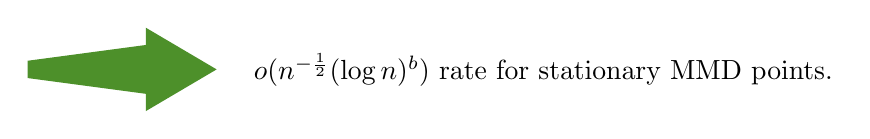
\begin{tikzpicture}[x=1cm,y=1cm]
            \fill[mmdGreen!85!yellow]
                (-3.95,0.26) -- (-2.45,0.46) -- (-2.45,0.68) -- (-1.55,0.15)
                -- (-2.45,-0.38) -- (-2.45,-0.16) -- (-3.95,0.04) -- cycle;

            \node[align=left, anchor=west] at (-1.20,0.14)
                {$o(n^{-\frac{1}{2}} (\log n)^b)$ rate for stationary MMD points.};
        \end{tikzpicture}
    \end{center}
    \begin{rem}
        If started with some point sets with $\operatorname{MMD}(\mu,\mu_n)=\calO(n^{-r})$, 
        then we can run MMD flow for $T=\calO(1)$ iterations to obtain a new point set with $o(n^{-r})$ rate. 
    \end{rem}
\end{frame}

\begin{frame}{Experiments}
    \begin{itemize}
        \item Mixture of Gaussians.
        \item KH is kernel herding~\citep{chen2012super}; KT is kernel thinning~\citep{dwivedi2024kernel}; SP is support points~\citep{mak2018support}. 
    \end{itemize}
    \vspace{0.2cm}
    \centering 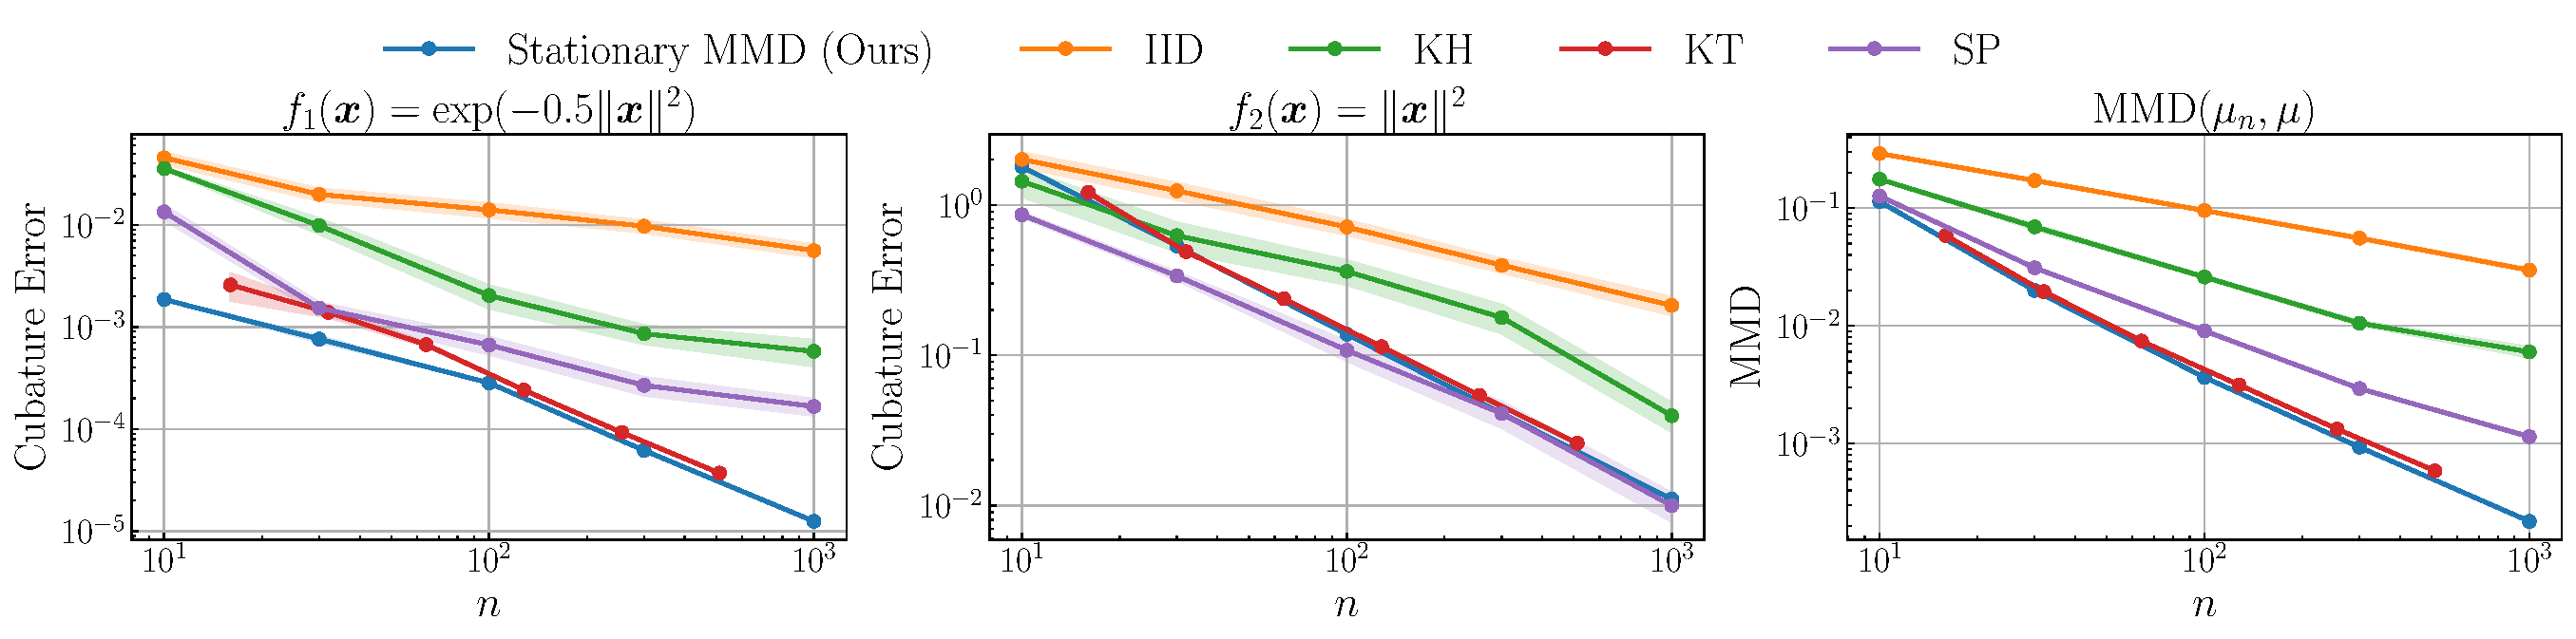
\includegraphics[width=\linewidth,keepaspectratio]{figures/mog.pdf}
    \vspace{-0.2cm}
    \begin{itemize}
        \item $f_1\in\calH$ while $f_2\notin\calH$.
        \item Stationary MMD points along with KT are the best.
        \item SP works well on $f_2$ since it uses $k(x,y)=\|x-y\|$.
    \end{itemize}
\end{frame}

\begin{frame}{Experiments}
    \begin{itemize}
        \item Coreset selection from a large dataset
        \item House (Top) has $22,784$ and Elevator (Bottom) has $16,599$ data points.
    \end{itemize}
    \vspace{0.1cm}
    \centering
    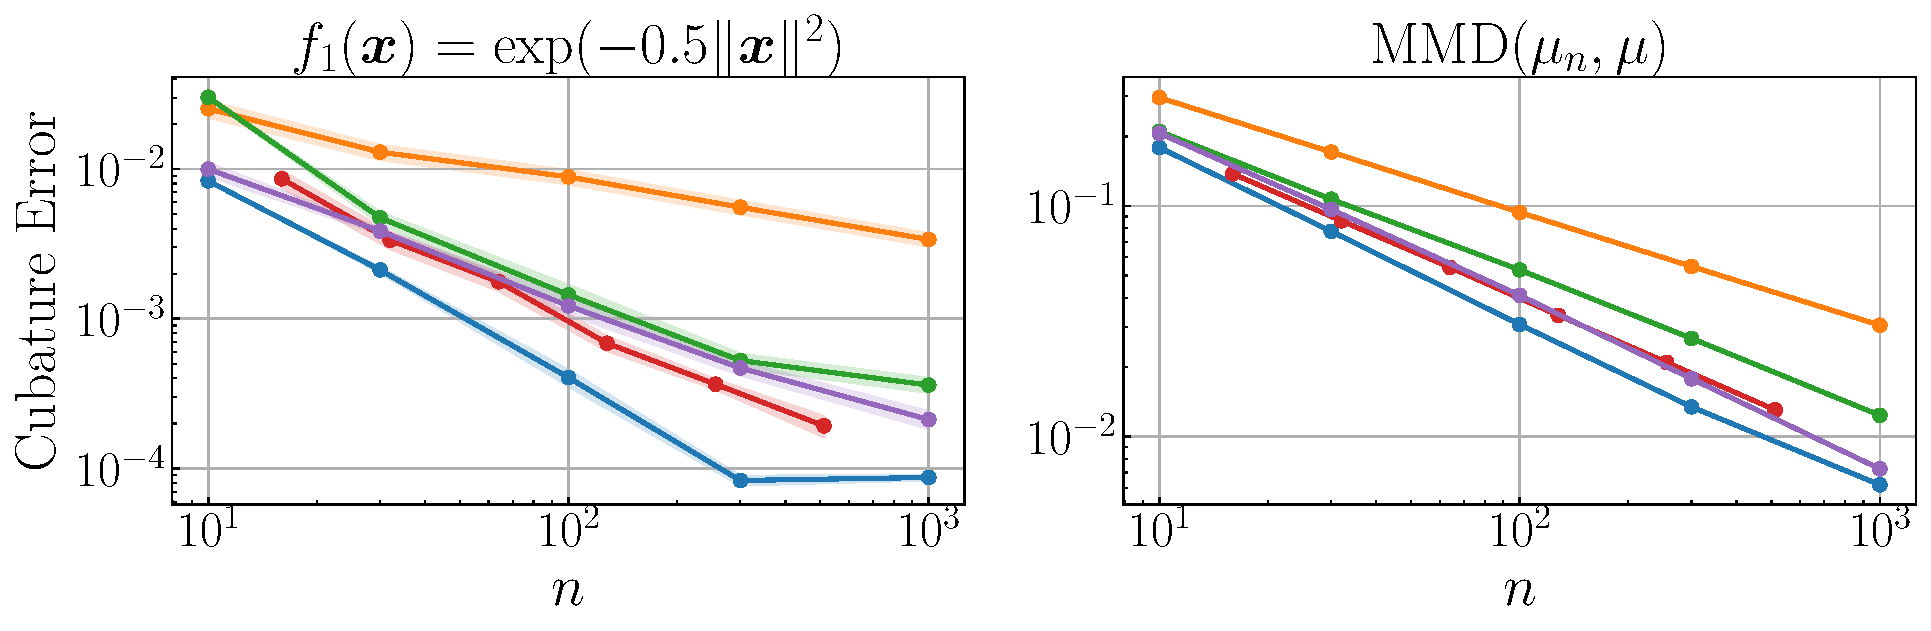
\includegraphics[width=0.65\linewidth,keepaspectratio]{figures/house.pdf}
    \vspace{0.1cm}
    \centering
    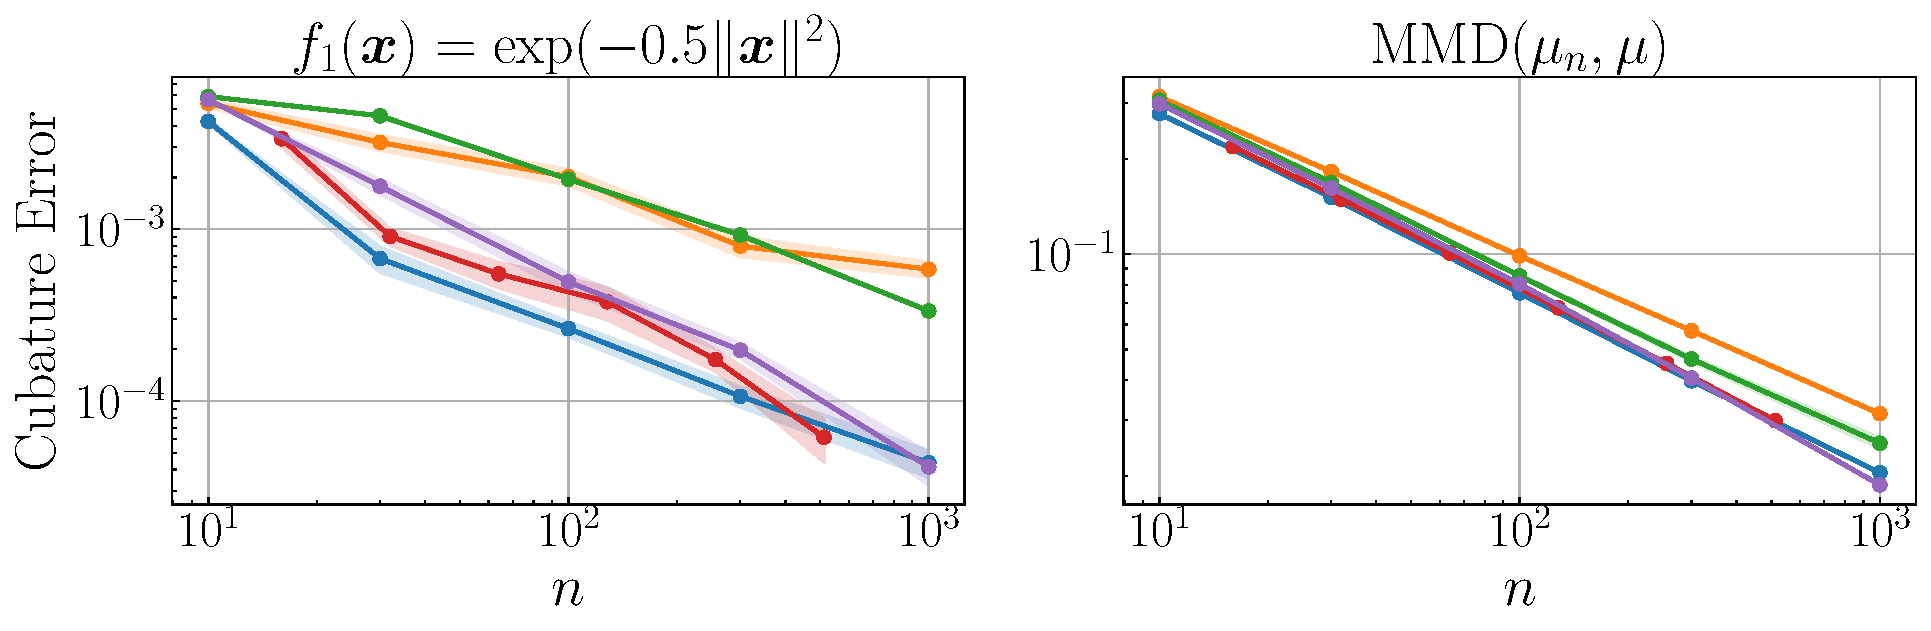
\includegraphics[width=0.65\linewidth,keepaspectratio]{figures/elevators.pdf}
\end{frame}

\begin{frame}{Summary}
    \begin{columns}[c,onlytextwidth]
        \column{0.68\textwidth}
            \begin{beamercolorbox}[wd=\linewidth, sep=0.35em, rounded=true]{answer box}
                {\bfseries Contributions}\\[-0.05cm]
                \begin{itemize}
                    \item We propose stationary MMD points.
                    \item A novel framework for low-discrepancy points.
                    \item Better rate from stationarity.
                \end{itemize}
            \end{beamercolorbox}
        \column{0.27\textwidth}
            \centering
            \resizebox{0.58\linewidth}{!}{\strengthcartoon}
    \end{columns}

    \vspace{0.28cm}

    \begin{columns}[c,onlytextwidth]
        \column{0.68\textwidth}
            \begin{beamercolorbox}[wd=\linewidth, sep=0.35em, rounded=true]{answer box}
                {\bfseries Limitations}\\[-0.05cm]
                \begin{itemize}
                    \item We only prove a $o(n^{-\frac{1}{2}} (\log n)^b)$ rate, unclear if better than IID $\calO(n^{-\frac{1}{2}})$ or not.
                    \item Noise injection in MMD flow is not ideal.
                \end{itemize}
            \end{beamercolorbox}
        \column{0.27\textwidth}
            \centering
            \resizebox{0.58\linewidth}{!}{\limitationcartoon}
    \end{columns}
\end{frame}
\begin{frame}[allowframebreaks]{References}
  \bibliographystyle{alpha}
  \bibliography{reference}
\end{frame}

\end{document}
